\documentclass{article}
\usepackage{amsmath,amssymb,amsthm}
\usepackage[margin=3cm]{geometry}
\usepackage{graphicx}
\usepackage{hyperref}

\renewcommand{\vec}[1]{\boldsymbol{#1}}
\newcommand{\unit}[1]{\,\hat{#1}}

\graphicspath{{./figures/}}

\begin{document}

\tableofcontents

\newpage

\section{Theme Areas}

\begin{enumerate}
\item Orbital mechanics --- vectors
  \begin{enumerate}
  \item shortest path between cities
  \item coordinate frames for observers on earth looking at satellites
  \item how does GPS work --- 4D solution for time/location
  \item angular frequency versus angular velocity
  \item solar days versus sidereal time
  \item where in the sky does the sun rise on a given date?
  \item how do we use the transit of Venus to compute the AU/km
    conversion --- parallax
  \end{enumerate}
\item Theme park rides and rollercoasters
  \begin{enumerate}
  \item G-forces felt by riders, how fast can we go without exceeding $-2g$/$+5g$?
  \item Speed needed to loop-the-loop
  \item Rollercoasters, swinging rides --- compute forces/moments in joints
  \end{enumerate}
\item Car dynamics
  \begin{enumerate}
  \item 2D side view of car, which direction are moments applied to
    wheels, forces of road on wheels, accelerating and braking, normal
    forces resulting --- why are front brakes better for braking, why
    are rear wheels better for accelerating? How do brake caliper
    forces translate to car deceleration?
  \item reconstructing accidents from tire marks on the road, sliding friction
  \item shape of roads, Euler spirals, don't use semi-circles, jerk
  \item banked roads, Untert\"urkheim track pictures
  \end{enumerate}
\item Sports and biomechanics
  \begin{enumerate}
  \item Bat/ball impacts, sweet spots
  \item Hitting in baseball, whole body unwind
  \item Long jump, max muscle forces, translate to jump length?
  \item Bicycle dynamics, lean, gyro forces?
  \item Ice skaters, twirling, angular momentum conservation
  \item Spin stabilization --- footballs, frisbees
  \end{enumerate}
\item Engines
  \begin{enumerate}
  \item gears, planetary gears
  \item vibration due to firing, piston movement, crankshaft rotation
  \item linkages in suspensions
  \end{enumerate}
\item Fluids, flying, sailing
  \begin{enumerate}
  \item lift and drag on airfoils, effects of angle of attack
  \item how do airfoils work? push air down, momentum change produces
    lift and drag
  \item sailboats --- how does sailing upwind work, importance of the
    keel, most efficient route with tacking?
  \item tangential/normal coordinates for fluid particles?
  \item helicopters --- role of the tail rotor, chinooks with two
    counter-rotating main rotors
  \end{enumerate}
\item Weapons
  \begin{enumerate}
  \item Projectile stabilization: Drag stabilization --- arrow
    fletching, spin stabilization --- rifling
  \item Siege weapons: catapults, trebuchets --- energy storage and
    transfer
  \item recurve bows, composite bows, longbows --- force profile
    versus draw distance and time after release --- total imparted
    impulse
  \item ballistic versus cruise missiles --- does the rotation of the
    Earth matter for ICBMs?
  \item how fast must a horizontal gun be fired to ensure that the
    bullet never lands?
  \item swords --- kinetic energy versus momentum, impulse of striking
  \end{enumerate}
\end{enumerate}

\section{Schedule}

Parallel each week:
\begin{enumerate}
\item Theme area
\item Skill drills
\item Derivations
\end{enumerate}

%%%%%%%%%%%%%%%%%%%%%%%%%%%%%%%%%%%%%%%%%%%%%%%%%%%%%%%%%%%%%%%%%%%%%%%%%%%%%%%

\section{Kinematics of Points}

\subsection{Positions and Coordinates}

A \emph{position} in 2D or 3D space is a single location, which may or
may not be occupied by a physical object. Positions exist before we
measure or describe them in any way, but to do calculations we need to
introduce coordinates for positions.

A \emph{coordinate chart} is a map that takes a position in space and
tells us what its \emph{coordinates} are. Coordinates serve to label
positions. For example, the coordinates ``5th Ave.\ and 42nd St.''
label the intersection next to the New York Public Library in the
street map coordinate chart. The coordinates of a position are a list
of scalars that act as a label for the position, such as $(x = 5, y =
42)$ for this position in New York.

It is common to have several different coordinate charts in use for
the same positions in space. For example, ``$40^\circ 45' 12.46''$N,
$73^\circ 58' 51.16''$W'' are also coordinates for this same
intersection, but this time in the latitude/longitude coordinate
chart, which we could write as the pair of scalars $(\lambda =
-73.980878, \phi = 40.753461)$\footnote{Here we converted
  degrees/minutes/seconds to decimal notation, wrote the coordinates
  in the East-West/North-South order to be horizontal/vertical, and
  realized that directions West are negative}.

\begin{center}
  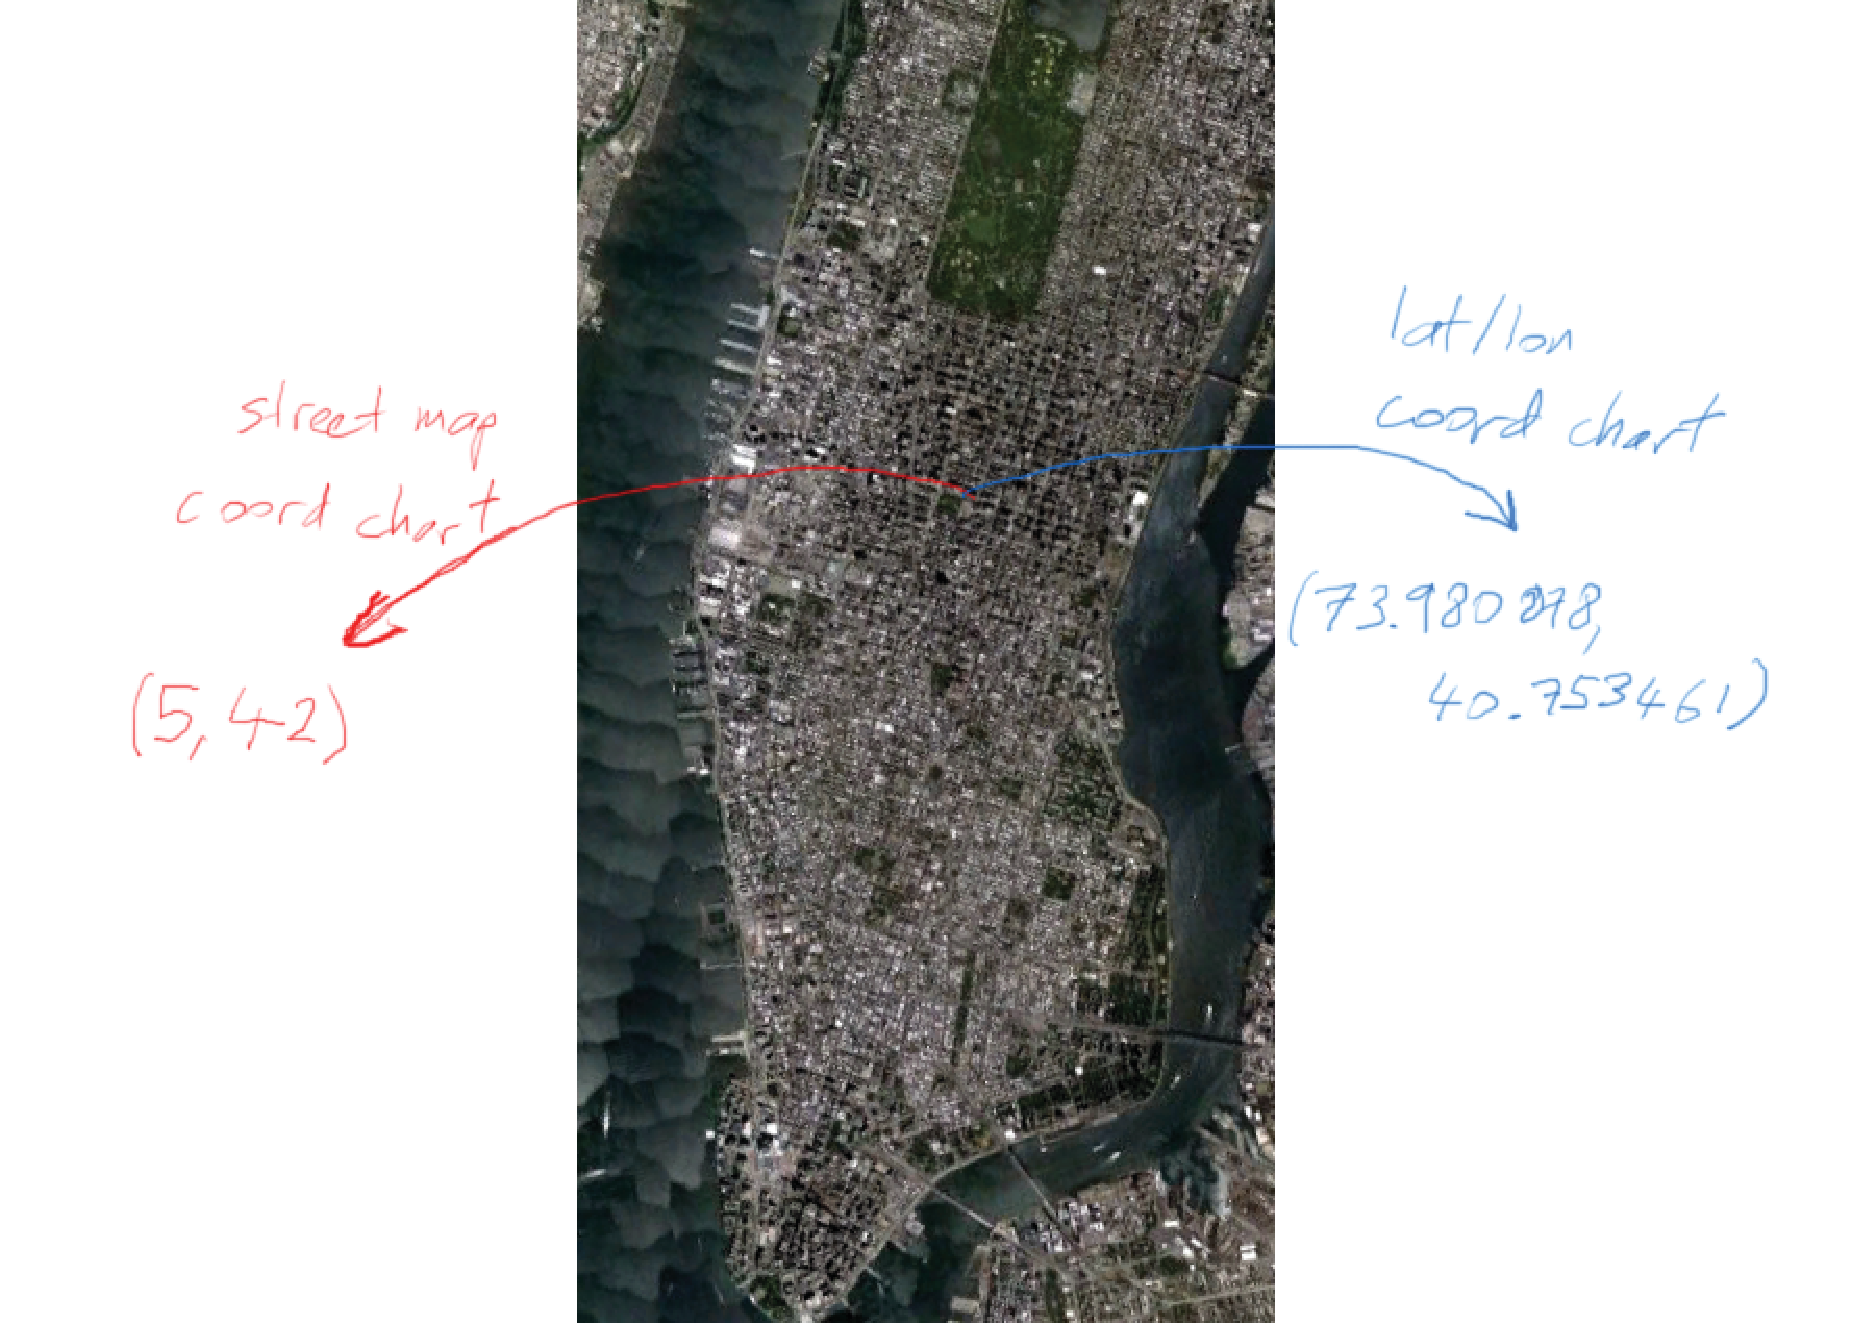
\includegraphics[width=8cm]{new_york_coords}
\end{center}

We can also think of a coordinate chart as mapping a list of
coordinates to a particular point, which is how we often illustrate a
coordinate chart graphically. For example, if we know a latitude and
longitude then we can locate the corresponding point on the Earth. The
\emph{origin} of a coordinate chart is the point with all zero
coordinates. Different coordinate charts may share an origin, or they
may have different origins.

If we have a point that moves around in space, then its coordinates
will change with time. It is also possible for the coordinate chart
itself to be moving in time, so that even if a point remains
stationary in space, its coordinates might be changing.

\paragraph{Example: Polar and Cartesian coordinates.} Show polar and
Cartesian coordinate lines, with different origins, moving particle,
show coords in both systems as functions of time. Ask: can the point
move somewhere so that both $(r, \theta) = (0,0)$ and $(x,y) = (0,0)$
simultaneously?

\paragraph{Example: Moving coordinate charts.} Same as previous
example, but moving coordinate charts with a stationary point.

When we describe a coordinate chart mathematically, we do so by
relating it to another coordinate chart (typically Cartesian).

\subsubsection{Cartesian Coordinates}

\subsubsection{Polar Coordinates}

\begin{align}
  x &= r \cos\theta & r &= \sqrt{x^2 + y^2} \\
  y &= r \sin\theta & \theta &= \operatorname{atan2}(y, x)
\end{align}

\subsubsection{Visualizing coordinate charts.}

To visualize a coordinate chart we will often draw the lines on which
just one of the coordinates is changing.

\paragraph{Example: Visualizing a coordinate chart.} Have an active
canvas on which we can draw with the mouse by clicking (just enable
drawing points? or also lines?). Have a readout showing the
coordinates of the mouse at all times. Use polar coordinates, which an
origin that is not centered on the canvas (or maybe some more complex
coordinate system?). Start with a blank canvas. Ask: draw points that
have first coordinate equal to 2. Then draw the points with first
coordinate equal to 1. Do the same for points with second coordinate
equal to 1, 2, 3, 4, 5, 6. What type of coordinate system is this?
Show the standard polar grid.

\subsection{Vectors and Bases}

A \emph{vector} is an arrow with a length and a direction. Just like
positions, vectors exist before we measure or describe them. Unlike
positions, vectors can mean many different things, such as position
vectors, velocities, etc. Vectors are not anchored to particular
positions in space, so we can slide a vector around and locate it at
any position.

\paragraph{Advanced aside:} Some textbooks differentiate between
\emph{free vectors}, which are free to slide around, and \emph{bound
  vectors}, which are anchored in space.

\paragraph{Notation:} We will write $\vec{v}$ to indicate a
vector. The length of $\vec{v}$ is written $v$.

\paragraph{Example V.PI:} show two vectors $v$ and $w$ and draw them at
several different positions each.

Vectors can be multiplied by a scalar number, which multiplies their
length. Vectors can also be added together, using the
\emph{parallelogram law of addition}.

\paragraph{Example V.PA:} parallelogram law of vector addition.

To describe vectors mathematically, we write them as a combination of
\emph{basis vectors}. An \emph{orthonormal basis} is a set of two (in
2D) or three (in 3D) basis vectors which are \emph{orthogonal} (have
$90^\circ$ angles between them) and {normal} (have length equal to
one)\footnote{We will not be using non-orthogonal or non-normal bases
  in this course.}. Any other vector can be written as a \emph{linear
  combination} of the basis vectors:
\begin{align}
  \vec{v} &= v_1 \unit{\i} + v_2 \unit{\j}
\end{align}
The numbers $v_1$ and $v_2$ are called the \emph{components} of
$\vec{v}$ in the $\unit{\i}, \unit{\j}$ basis.

\paragraph{Example V.BS:} Show a vector $\vec{v}$ and two different bases
$\unit{\i}, \unit{\j}$ and $\unit{a}, \unit{b}$ and show the components. From
now on, always have $\unit{\i}, \unit{\j}$ being the regular axis-aligned
basis and $\unit{a}, \unit{b}$ being rotated by $\pi/4$.

\paragraph{Image quiz:} Show the same basis twice, once as a regular
pair connected at the origin, one where the basis vectors are
disconnected. Ask if these are the same basis.

\subsubsection{Length of Vectors}

The length of a vector $\vec{v}$ is written either $\|\vec{v}\|$ or
just plain $v$. The length can be computed using \emph{Pythagorus'
  theorem}:
\begin{align}
  \vec{v} &= v_1 \unit{i} + v_2 \unit{j} \\
  v = \|\vec{v}\| &= \sqrt{v_1^2 + v_2^2}
\end{align}

\paragraph{Important point:} The formula $v = \sqrt{v_1^2 + v_2^2}$
only works if the components are from a single orthonormal basis.

\paragraph{Example:} If $\vec{v} = 3\unit{\i} + 4\unit{a}$, what is $v$?
Answer: not $\sqrt{3^2 + 4^2}$. Instead, it is \ldots.

\paragraph{Example: Triangle inequality.} If $\vec{u} = \vec{v} +
\vec{w}$, how are the lengths $u, v, w$ related? Show picture. Answer:
certainly it is not true that $u = v + w$. Instead it is true that $u
\le v + w$. There is no way that $u$ can be longer than the combined
lengths of $v$ and $w$, and it will only be equal if $v$ and $w$ are
in the same direction.

\subsubsection{Unit vectors}

Defines the direction of $\vec{v}$.

\begin{align}
  \hat{v} = \frac{\vec{v}}{v}
\end{align}

Any vector can be written as:
\begin{align}
  \vec{v} = v \hat{v}
\end{align}
Here $v$ is the length, $\hat{v}$ is the direction unit vector.

\subsubsection{Dot Product}

\begin{align}
  \vec{u} \cdot \vec{v} &= u v \cos\theta
\end{align}
Squared length:
\begin{align}
  v^2 &= \vec{v} \cdot \vec{v}
\end{align}

Length and angle from dot product:
\begin{align}
  v &= \sqrt{\vec{v} \cdot \vec{v}} \\
  \cos\theta &= \frac{\vec{u} \cdot \vec{v}}{u v}
\end{align}

\paragraph{Example: Parallelogram area.} $\vec{u} \cdot \vec{v}$ is
the area of the parallelogram formed by $\vec{u}$ and $\vec{v}$.

\paragraph{Example: Finding great-circle distance between cities.}
Take lat/long for Urbana and Perth, say. We want to know great-circle
distance. Convert lat/long/R to xyz position vectors from earth
center. Consider great circle plane and great circle, that contains
these two vectors. The angle on this plane is the angle between the
vectors. Find this from the dot product. Find distance with $s = R
\theta$. Make the note that this is very hard to do directly from
lat/long without switching to xyz and using vectors.

\paragraph{Example V.OR: Finding orthogonal vectors.} If $\vec{u} = u_1
\unit{\i} + u_2 \unit{\j}$, then $\vec{v} = - u_2 \unit{\i} + u_1
\unit{\j}$ is orthogonal, as is $\vec{w} = u_2 \unit{\i} - u_1
\unit{\j} = -\vec{v}$. This doesn't work in 3D!

\subsubsection{Cross Product}

\begin{align}
  \vec{w} &= \vec{u} \times \vec{v} \\
  &= (u_2 v_3 - u_3 v_2) \unit{\i}
  + (u_3 v_1 - u_1 v_3) \unit{\j}
  + (u_1 v_2 - u_2 v_1) \unit{k} \\
  w &= u v \sin\theta \\
  \vec{w} \cdot \vec{u} = \vec{w} \cdot \vec{v} &= 0
\end{align}

\paragraph{Example: Satellite positions.} Take ISS. Assume we have xyz
position $\vec{r}$ of ISS at time zero, and also we know xyz normal
vector $\vec{n}$, all in an inertial frame. We also know orbital
period $T$. We want to work out where the ISS is in 1 hour, say. Do
this by finding a basis consisting of $\vec{r}, \vec{n}, \vec{a} =
\vec{n} \times \vec{r}$. In this basis the ISS moves in the
$\vec{r}$-$\vec{a}$ plane with angular velocity $2\pi / T$ starting
from $(R,0,0)$. Find position in this basis at later time. Convert
back to xyz.

\paragraph{Useful formulas:}
\begin{itemize}
\item Antisymmetry:
  \begin{align}
    \vec{u} \times \vec{v} = - \vec{v} \times \vec{u}
  \end{align}
  Derivation: Write out both sides in components.
\item $\vec{u} \times \vec{u} = 0$ (Derivation: from antisymmetry)
\item Bilinearity:
  \begin{align}
    \vec{a} \times (\vec{b} + \vec{c})
    &= \vec{a} \times \vec{b} + \vec{a} \times \vec{c} \\
    (\vec{a} + \vec{b}) \times \vec{c}
    &= \vec{a} \times \vec{c} + \vec{b} \times \vec{c} \\
    \vec{a} \times (\beta \vec{b}) &= \beta (\vec{a} \times \vec{b}) = (\beta \vec{a}) \times \vec{b}
  \end{align}
  Derivation: Write out both sides in components.
\item Scalar triple product: $\vec{u} \cdot (\vec{v} \times \vec{w})$
  is the volume of the parallelepiped defined by $\vec{u}, \vec{v},
  \vec{w}$. It satisfies the scalar triple product formula:
  \begin{align}
    \vec{u} \cdot (\vec{v} \times \vec{w})
    = \vec{v} \cdot (\vec{w} \times \vec{u})
    = \vec{w} \cdot (\vec{u} \times \vec{v})
  \end{align}
  Derivation: write first two expressions out in components and check
  that they give the same result:
  \begin{align}
    \vec{u} \cdot (\vec{v} \times \vec{w})
    &= (u_1 \unit{\i} + u_2 \unit{\j} + u_3 \unit{k})
    \cdot \big( (v_1 \unit{\i} + v_2 \unit{\j} + v_3 \unit{k})
    \times (w_1 \unit{\i} + w_2 \unit{\j} + w_3 \unit{k}) \big) \\
    &= (u_1 \unit{\i} + u_2 \unit{\j} + u_3 \unit{k}) \cdot \big(
    (v_2 w_3 - v_3 w_2) \unit{\i}
    + (v_3 w_1 - v_1 w_3) \unit{\j}
    + (v_1 w_2 - v_2 w_1) \unit{k} \big) \\
    &= u_1 v_2 w_3 - u_1 v_3 w_2
    + u_2 v_3 w_1 - u_2 v_1 w_3
    + u_3 v_1 w_2 - u_3 v_2 w_1 \\
    \vec{v} \cdot (\vec{w} \times \vec{u})
    &= (v_1 \unit{\i} + v_2 \unit{\j} + v_3 \unit{k})
    \cdot \big( (w_1 \unit{\i} + w_2 \unit{\j} + w_3 \unit{k})
    \times (u_1 \unit{\i} + u_2 \unit{\j} + u_3 \unit{k}) \big) \\
    &= (v_1 \unit{\i} + v_2 \unit{\j} + v_3 \unit{k}) \cdot \big(
    (w_2 u_3 - w_3 u_2) \unit{\i}
    + (w_3 u_1 - w_1 u_3) \unit{\j}
    + (w_1 u_2 - w_2 u_1) \unit{k} \big) \\
    &= v_1 w_2 u_3 - v_1 w_3 u_2
    + v_2 w_3 u_1 - v_2 w_1 u_3
    + v_3 w_1 u_2 - v_3 w_2 u_1
  \end{align}
  The third expression is also the same.
\item Vector triple product is $\vec{a} \times (\vec{b} \times
  \vec{c})$. Vector triple product expansion:
  \begin{align}
    \vec{a} \times (\vec{b} \times \vec{c})
    = (\vec{a} \cdot \vec{c}) \vec{b} - (\vec{a} \cdot \vec{b}) \vec{c}
  \end{align}
  Derivation: In components:
  \begin{align}
    \vec{a} \times (\vec{b} \times \vec{c})
    &= (a_1 \unit{\i} + a_2 \unit{\j} + a_3 \unit{k})
    \times \Big(
    (b_1 \unit{\i} + b_2 \unit{\j} + b_3 \unit{k})
    \times (c_1 \unit{\i} + c_2 \unit{\j} + c_3 \unit{k}) \Big) \\
    &= (a_1 \unit{\i} + a_2 \unit{\j} + a_3 \unit{k})
    \times \Big(
    (b_2 c_3 - b_3 c_2) \unit{\i}
    + (b_3 c_1 - b_1 c_3) \unit{\j}
    + (b_1 c_2 - b_2 c_1) \unit{k} \Big) \\
    &= \Big(a_2 (b_1 c_2 - b_2 c_1) - a_3 (b_3 c_1 - b_1 c_3)\Big) \unit{\i} \\
    &\quad+ \Big(a_3 (b_2 c_3 - b_3 c_2) - a_1 (b_1 c_2 - b_2 c_1)\Big) \unit{\j} \\
    &\quad+ \Big(a_1 (b_3 c_1 - b_1 c_3) - a_2 (b_2 c_3 - b_3 c_2)\Big) \unit{k} \\
    &= (a_2 b_1 c_2 - a_2 b_2 c_1 - a_3 b_3 c_1 + a_3 b_1 c_3) \unit{\i} \\
    &\quad+ (a_3 b_2 c_3 - a_3 b_3 c_2 - a_1 b_1 c_2 + a_1 b_2 c_1) \unit{\j} \\
    &\quad+ (a_1 b_3 c_1 - a_1 b_1 c_3 - a_2 b_2 c_3 + a_2 b_3 c_2) \unit{k} \\
    &= (a_1 b_1 c_1 + a_2 b_1 c_2 + a_3 b_1 c_3 - a_1 b_1 c_1 - a_2 b_2 c_1 - a_3 b_3 c_1) \unit{\i} \\
    &\quad+ (a_1 b_2 c_1 + a_2 b_2 c_2 + a_3 b_2 c_3 - a_1 b_1 c_2 - a_2 b_2 c_2 - a_3 b_3 c_2) \unit{\j} \\
    &\quad+ (a_1 b_3 c_1 + a_2 b_3 c_2 + a_3 b_3 c_3 - a_1 b_1 c_3 - a_2 b_2 c_3 - a_3 b_3 c_3) \unit{k} \\
    &= (a_1 b_1 + a_2 c_2 + a_3 c_3) b_1 \unit{\i}
    + (a_1 c_1 + a_2 c_2 + a_3 c_3) b_2 \unit{\j}
    + (a_1 c_1 + a_2 c_2 + a_3 c_3) b_3 \unit{k} \\
    &\quad- (a_1 b_1 + a_2 b_2 + a_3 b_3) c_1 \unit{\i}
    - (a_1 b_1 + a_2 b_2 + a_3 b_3) c_2 \unit{\j}
    - (a_1 b_1 + a_2 b_2 + a_3 b_3) c_3 \unit{k} \\
    &= (\vec{a} \cdot \vec{c}) \vec{b} - (\vec{a} \cdot \vec{b}) \vec{c}
  \end{align}
\item Cross product orthogonality:
  \begin{align}
    \vec{a} \times \vec{b} \text{ is orthogonal to } \vec{a} \text{ and } \vec{b}
  \end{align}
  Derivation: follows immediately from the scalar triple product formula:
  \begin{align}
    \vec{a} \cdot (\vec{a} \times \vec{b})
    = \vec{b} \cdot (\vec{a} \times \vec{a}) = 0
  \end{align}
  and similarly for $\vec{b}$.
\item Binet-Cauchy identity:
  \begin{align}
    (\vec{a} \times \vec{b}) \cdot (\vec{c} \times \vec{d})
    = (\vec{a} \cdot \vec{c})(\vec{b} \cdot \vec{d})
    - (\vec{a} \cdot \vec{d})(\vec{b} \cdot \vec{c})
  \end{align}
  Derivation: From the scalar triple product formula and the vector
  triple product expansion:
  \begin{align}
    (\vec{a} \times \vec{b}) \cdot (\vec{c} \times \vec{d})
    &= \vec{c} \cdot \big( \vec{d} \times (\vec{a} \times \vec{b}) \big) \\
    &= \vec{c} \cdot \big( (\vec{d} \cdot \vec{b}) \vec{a}
    - (\vec{d} \cdot \vec{a}) \vec{b} \big) \\
    &= (\vec{d} \cdot \vec{b}) (\vec{c} \cdot \vec{a})
    - (\vec{d} \cdot \vec{a}) (\vec{c} \cdot \vec{b})
  \end{align}
\item Lagrange's identity:
  \begin{align}
    \| \vec{a} \times \vec{b} \|^2 = \|\vec{a}\|^2 \|\vec{b}\|^2 -
    (\vec{a} \cdot \vec{b})^2
  \end{align}
  Derivation: Follows immediately from the Binet-Cauchy identity.
\item Cross product length:
  \begin{align}
    \| \vec{a} \times \vec{b} \| = \|\vec{a}\| \|\vec{b}\| \sin\theta
  \end{align}
  Derivation: From Lagrange's identity:
  \begin{align}
    \| \vec{a} \times \vec{b} \|^2
    &= \|\vec{a}\|^2 \|\vec{b}\|^2 - (\vec{a} \cdot \vec{b})^2 \\
    &= \|\vec{a}\|^2 \|\vec{b}\|^2 - (\|\vec{a}\| \|\vec{b}\| \cos\theta)^2 \\
    &= \|\vec{a}\|^2 \|\vec{b}\|^2 (1 - \cos^2\theta) \\
    &= \|\vec{a}\|^2 \|\vec{b}\|^2 \sin^2\theta
  \end{align}
\item Jacobi's identity:
  \begin{align}
    \vec{a} \times (\vec{b} \times \vec{c})
    + \vec{b} \times (\vec{c} \times \vec{a})
    + \vec{c} \times (\vec{a} \times \vec{b})
    = 0
  \end{align}
  Derivation: Using the vector triple product expansion:
  \begin{align}
    &\vec{a} \times (\vec{b} \times \vec{c})
    + \vec{b} \times (\vec{c} \times \vec{a})
    + \vec{c} \times (\vec{a} \times \vec{b}) \\
    &\qquad= (\vec{a} \cdot \vec{c}) \vec{b} - (\vec{a} \cdot \vec{b}) \vec{c}
    + (\vec{b} \cdot \vec{a}) \vec{c} - (\vec{b} \cdot \vec{c}) \vec{a}
    + (\vec{c} \cdot \vec{b}) \vec{a} - (\vec{c} \cdot \vec{a}) \vec{b} \\
    &\qquad= 0
  \end{align}
\item Quadruple vector product expansion:
  \begin{align}
    (\vec{a} \times \vec{b}) \times (\vec{a} \times \vec{c})
    = \big( \vec{a} \cdot (\vec{b} \times \vec{c}) \big) \vec{a}
  \end{align}
  Derivation: Take $\vec{d} = (\vec{a} \times \vec{b}) \times (\vec{a}
  \times \vec{c})$. Then $\vec{d}$ is in the $\vec{a},\vec{b}$ plane
  and in the $\vec{a},\vec{c}$ plane, so it is a scalar multiple of
  $\vec{a}$. We use the scalar triple product formula and the vector
  triple product expansion to compute:
  \begin{align}
    \vec{d} \cdot \vec{a}
    &= \vec{a} \cdot \big( (\vec{a} \times \vec{b})
    \times (\vec{a} \times \vec{c}) \big) \\
    &= (\vec{a} \times \vec{c}) \cdot
    \big( \vec{a} \times (\vec{a} \times \vec{b}) \big) \\
    &= (\vec{a} \times \vec{c}) \cdot
    \big( (\vec{a} \cdot \vec{b}) \vec{a}
    - (\vec{a} \cdot \vec{a}) \vec{b} \big) \\
    &= - (\vec{a} \cdot \vec{a})
    \vec{b} \cdot (\vec{a} \times \vec{c}) \\
    &= (\vec{a} \cdot \vec{a})
    \big( \vec{a} \cdot (\vec{b} \times \vec{c}) \big)
  \end{align}
  Then
  \begin{align}
    \vec{d} = \operatorname{Proj}(\vec{d}, \vec{a})
    = \left(\frac{\vec{d} \cdot \vec{a}}{\vec{a} \cdot \vec{a}}\right)
    \vec{a}
    = \big( \vec{a} \cdot (\vec{b} \times \vec{c}) \big) \vec{a}
  \end{align}
\end{itemize}

\subsubsection{Projection and Rejection}

\begin{align}
  \operatorname{Proj}(\vec{u}, \vec{v})
  &= (\vec{u} \cdot \hat{v}) \hat{v}
  = \left(\frac{\vec{u} \cdot \vec{v}}{v^2}\right) \vec{v}
  = \left(\frac{\vec{u} \cdot \vec{v}}{\vec{v} \cdot \vec{v}}\right) \vec{v} \\
  \operatorname{Rej}(\vec{u}, \vec{v})
  &= \vec{u} - \operatorname{Proj}(\vec{u}, \vec{v})
  = \vec{u} - (\vec{u} \cdot \hat{v}) \hat{v}
  = \vec{u} - \left(\frac{\vec{u} \cdot \vec{v}}{v^2}\right) \vec{v}
  = \vec{u} - \left(\frac{\vec{u} \cdot \vec{v}}{\vec{v} \cdot \vec{v}}\right) \vec{v}
\end{align}

\subsubsection{Changing bases}

\paragraph{Important point:} Vector expressions are true no matter
which basis we write the vectors in, even if they are written in
different bases.

\paragraph{Example V.CB:} $\vec{w} = \vec{u} + 2 \vec{v}$, draw the
image. This is true no matter which bases are being used for $\vec{u}$
and $\vec{v}$. For example, even if we use different bases: $\vec{u} =
3\unit{\i} + 2\unit{\j}$ and $\vec{v} = 5\unit{a} - \unit{b}$, then $\vec{w} =
3\unit{\i} + 2\unit{\j} + 10\unit{a} - 2\unit{b}$ is true. Of course, we would
normally convert these to a single basis, but we don't have to.

To change the basis that a vector is written in, we need to know how
the basis vectors are related. For example, if we have $\vec{v} =
3\unit{\i} + 2\unit{\j}$ and we want to write this in the $\unit{a}, \unit{b}$
basis, then we need to know $\unit{\i}, \unit{\j}$ in terms of $\unit{a}, \unit{b}$. For example,
\begin{align}
  \unit{\i} &= \frac{1}{\sqrt{2}} \unit{a} - \frac{1}{\sqrt{2}} \unit{b} \\
  \unit{\j} &= \frac{1}{\sqrt{2}} \unit{a} + \frac{1}{\sqrt{2}} \unit{b}
\end{align}
Then we can substitute and re-arrange:
\begin{align}
  \vec{v} &= 3\unit{\i} + 2\unit{\j} \\
  &= 3\left(\frac{1}{\sqrt{2}} \unit{a} - \frac{1}{\sqrt{2}} \unit{b}\right)
  + 2\left(\frac{1}{\sqrt{2}} \unit{a} + \frac{1}{\sqrt{2}} \unit{b}\right) \\
  &= \left(\frac{3}{\sqrt{2}} + \frac{2}{\sqrt{2}} \right) \unit{a}
  + \left(-\frac{3}{\sqrt{2}} + \frac{2}{\sqrt{2}} \right) \unit{b} \\
  &= \frac{5}{\sqrt{2}} \unit{a} - \frac{1}{\sqrt{2}} \unit{b}
\end{align}
If we want to convert back the other way then we would need to know
$\unit{a}, \unit{b}$ in terms of $\unit{\i}, \unit{\j}$. We can find this by
solving for $\unit{a}, \unit{b}$ above.

\paragraph{Example:} $\vec{w} = \vec{u} \times \vec{v}$, same as
above: $\vec{u} = 3\unit{\i} + 2\unit{\j}$ and $\vec{v} = 5\unit{a} -
\unit{b}$. Then $\vec{w} = 15 \unit{\i} \times \unit{a} - 3 \unit{\i}
\times \unit{b} + 10 \unit{\j} \times \unit{a} - 2 \unit{\j} \times
\unit{b}$. Work out what these are individually. Take $\unit{a},
\unit{b}$ rotated by $\pi/4$ from $\unit{\i}, \unit{\j}$, so we can do
the cross products by hand or something?

\subsubsection{Time-dependent vectors and bases}

We can have dynamic vectors which change over time, so their
components also change. Alternatively, we can have a fixed vector but
dynamic basis.

\paragraph{Example V.CV:} Show a lengthening and rotating vector and
how its components change over time in a fixed basis.

\paragraph{Example V.RB:} Show a fixed vector, but a rotating basis,
and how the components change over time.

\subsubsection{Basis vectors from different coordinate systems}

polar coordinates:
\begin{align}
  \unit{r} &= \cos\theta \unit{\i} + \sin\theta \unit{\j} \\
  \unit{\theta} &= - \sin\theta \unit{\i} + \cos\theta \unit{\j}
\end{align}

\subsection{Calculus and Vectors}

Time-dependent vectors can be differentiated in exactly the same way
that we differentiate scalar functions. For a time-dependent vector
$\vec{v}(t)$, the derivative $\dot{\vec{v}}(t)$ is
\begin{align}
  \dot{\vec{v}}(t) &= \frac{d}{dt} \vec{v}(t)
  = \lim_{\Delta t \to 0}
  \frac{\vec{v}(t + \Delta t) - \vec{v}(t)}{\Delta t}
\end{align}

\paragraph{Example V.DV: Vector derivatives.} Show a vector $\vec{v}(t)$
with a fixed origin and the end tracing out a curved path (path is
shown as a dotted line). Show $\vec{v}(t)$ animated. Then show
$\vec{v}(t + \Delta t)$ and the construction for the derivative,
resulting in the derivative vector.

\paragraph{Notation:} We will use either the dot notation
$\dot{\vec{v}}(t)$ or the full derivative notation
$\frac{d\vec{v}(t)}{dt}$, depending on which is clearer and more
convenient. We will often not write the time dependency explicitly, so
we might write just $\dot{\vec{v}}$ or $\frac{d\vec{v}}{dt}$.

In a fixed basis we differentiate a vector by differentiating each
component:
\begin{align}
  \vec{v}(t) &= v_1(t) \unit{\i} + v_2(t) \unit{\j} \\
  \dot{\vec{v}}(t) &= \dot{v}_1(t) \unit{\i} + \dot{v}_2(t) \unit{\j}
\end{align}

\paragraph{Example: Differentiating vectors component-wise (fixed basis).} Show the
sample example as above, but now show the $v_1$ and $v_2$ components
of $\vec{v}$. Turn on derivatives of each component and show how they
sum to give the vector derivative.

\paragraph{Derivation:}
\begin{align}
  \vec{v}(t) &= v_1(t) \unit{\i} + v_2(t) \unit{\j} \\
  \dot{\vec{v}}(t) &= \lim_{\Delta t \to 0}
  \frac{\vec{v}(t + \Delta t) - \vec{v}(t)}{\Delta t} \\
  &= \lim_{\Delta t \to 0}
  \frac{(v_1(t + \Delta t) \unit{\i} + v_2(t + \Delta t) \unit{\j})
    - (v_1(t) \unit{\i} + v_2(t) \unit{\j})}{\Delta t} \\
  &= \lim_{\Delta t \to 0}
  \frac{(v_1(t + \Delta t) - v_1(t)) \unit{\i}
    + (v_2(t + \Delta t) - v_2(t)) \unit{\j}}{\Delta t} \\
  &= \left(\lim_{\Delta t \to 0}
    \frac{v_1(t + \Delta t) - v_1(t)}{\Delta t} \right) \unit{\i}
  + \left(\lim_{\Delta t \to 0}
    \frac{v_2(t + \Delta t) - v_2(t) }{\Delta t}\right) \unit{\j} \\
  &= \dot{v}_1(t) \unit{\i} + \dot{v}_2(t) \unit{\j}
\end{align}

We can also differentiate vector expressions, such as dot products and
cross products. These act like multiplication, so the \emph{product
  rule} applies:
\begin{align}
  \frac{d}{dt}(\vec{v} \cdot \vec{u})
  &= \dot{\vec{v}} \cdot \vec{u} + \vec{v} \cdot \dot{\vec{u}} \\
  \frac{d}{dt}(\vec{v} \times \vec{u})
  &= \dot{\vec{v}} \times \vec{u} + \vec{v} \times \dot{\vec{u}}
\end{align}

\paragraph{Example: Differentiating complex vector expressions.} What
is $\frac{d}{dt} \big( \vec{u} \cdot (\vec{v} + \vec{v} \times
\vec{w}) \big)$?
\begin{align}
  \frac{d}{dt} \big( \vec{u} \cdot
  (\vec{v} + \vec{v} \times \vec{w}) \big)
  &= \dot{\vec{u}} \cdot 
  (\vec{v} + \vec{v} \times \vec{w})
  + \vec{u} \cdot \frac{d}{dt}
  (\vec{v} + \vec{v} \times \vec{w}) \\
  &= \dot{\vec{u}} \cdot 
  (\vec{v} + \vec{v} \times \vec{w})
  + \vec{u} \cdot (\dot{\vec{v}}
  + \dot{\vec{v}} \times \vec{w} + \vec{v} \times \dot{\vec{w}})
\end{align}

We can break a vector derivative down into the change in length and
the change in direction:
\begin{align}
  \vec{v} &= v \hat{v} \\
  \dot{\vec{v}} &= \dot{v} \hat{v} + v \dot{\hat{v}}
\end{align}
To compute the derivative of length and direction we can use:
\begin{align}
  \dot{v} &= \dot{\vec{v}} \cdot \hat{v} \\
  \hat{v} &= \frac{1}{v} \operatorname{Rej}(\dot{\vec{v}}, \hat{v})
\end{align}
This means that
\begin{align}
  \dot{v} \hat{v} &= (\dot{\vec{v}} \cdot \hat{v}) \hat{v}
  = \operatorname{Proj}(\dot{\vec{v}}, \vec{v}) \\
  v \dot{\hat{v}} &= v \frac{1}{v} \operatorname{Rej}(\dot{\vec{v}}, \hat{v})
  = \operatorname{Rej}(\dot{\vec{v}}, \hat{v})
\end{align}
So the decomposition is
\begin{align}
  \dot{\vec{v}} &= \underbrace{\dot{v}
    \hat{v}}_{\operatorname{Proj}(\dot{\vec{v}}, \vec{v})} +
  \underbrace{v \dot{\hat{v}}}_{\operatorname{Rej}(\dot{\vec{v}},
    \hat{v})}
\end{align}

\paragraph{Derivation:}
For length:
\begin{align}
  v &= \sqrt{\vec{v} \cdot \vec{v}} \\
  \frac{d}{dt} v &= \frac{d}{dt} \big( (\vec{v} \cdot \vec{v})^{1/2} \big) \\
  \dot{v} &= \frac{1}{2} (\vec{v} \cdot \vec{v})^{-1/2}
  (\dot{\vec{v}} \cdot \vec{v} + \vec{v} \cdot \dot{\vec{v}}) \\
  &= \frac{1}{2\sqrt{v^2}} (2 \dot{\vec{v}} \cdot \vec{v}) \\
  &= \dot{\vec{v}} \cdot \hat{v}
\end{align}

\paragraph{Derivation:}
For direction:
\begin{align}
  \hat{v} &= \frac{\vec{v}}{v} \\
  \frac{d}{dt} \hat{v} &= \frac{d}{dt}\left(\frac{\vec{v}}{v}\right) \\
  \dot{\hat{v}} &= \frac{\dot{\vec{v}} v - \vec{v} \dot{v}}{v^2} \\
  &= \frac{\dot{\vec{v}}}{v}
  - \frac{\dot{\vec{v}} \cdot \hat{v}}{v^2} \vec{v} \\
  &= \frac{1}{v} \big( \dot{\vec{v}}
  - (\dot{\vec{v}} \cdot \hat{v}) \hat{v} \big)\\
  &= \frac{1}{v} \operatorname{Rej}(\dot{\vec{v}}, \hat{v})
\end{align}

\paragraph{Example V.DD: Changing length and direction.} Show the same
vector derivative example as before, but decompose the derivative into
$\hat{v}$ and $\dot{\hat{v}}$ components. Show the projections.

\subsection{Rotations and Angular Velocity}

A \emph{rotation} of a vector is a change which only alters the
direction, not the length, of a vector. A rotation consists of a
\emph{rotation axis} and a \emph{rotation rate}. By taking the
rotation axis as a direction and the rotation rate as a length, we can
write the rotation as a vector, known as the \emph{angular velocity
  vector} $\vec{\omega}$. We use the \emph{right-hand-rule} to
describe the direction of rotation.

\paragraph{Example:} Show a cloud of vectors rotating in 3D around an
angular velocity vector. Maybe have the angular velocity vector change
in length, showing the rotation slowing down and speeding up. Maybe
also have it change in direction, showing the rotation axis change.

In 2D the angular velocity can be thought of as a scalar (positive for
counter-clockwise, negative for clockwise). This scalar is just the
out-of-plane component of the full angular velocity vector. We can
draw the angular velocity as either a vector pointing out of the
plane, or as a circle-arrow in the plane, which is simpler for 2D
diagrams.

\paragraph{Example:} Show a set of 2D vectors rotating in the plane,
with the angular velocity shown as an out-of-plane vector and an
in-plane circle-arrow.

If a vector $\vec{v}$ is rotating with angular velocity vector
$\vec{\omega}$, the rate of change of $\vec{v}$ is
\begin{align}
  \dot{\vec{v}} &= \vec{\omega} \times \vec{v}
\end{align}
We will see below that this is correct.

\subsubsection{Properties of rotations}

\begin{itemize}
\item Vector derivatives due to rotation are orthogonal to the vector:
  \begin{align}
    \dot{\vec{v}} \cdot \vec{v} = 0
  \end{align}
  Derivation: Using the scalar triple product formula:
  \begin{align}
    \vec{v} \cdot \dot{\vec{v}}
    &= \vec{v} \cdot \big( \vec{\omega} \times \vec{v} \big)
    &= \vec{\omega} \cdot \big( \vec{v} \times \vec{v} \big)
    &= 0
  \end{align}
\item If we have two vectors $\vec{u}$ and $\vec{v}$ both rotating
  with an angular velocity $\vec{\omega}$, then $\vec{u} \cdot
  \vec{v}$ is constant:
  \begin{align}
    \frac{d}{dt} \big( \vec{u} \cdot \vec{v} \big) = 0
  \end{align}
  Derivation: Using the scalar triple product formula:
  \begin{align}
    \frac{d}{dt} \big( \vec{u} \cdot \vec{v} \big)
    &= \dot{\vec{u}} \cdot \vec{v} + \vec{u} \cdot \dot{\vec{v}} \\
    &= (\vec{\omega} \times \vec{u}) \cdot \vec{v}
    + \vec{u} \cdot (\vec{\omega} \times \vec{v}) \\
    &= \vec{v} \cdot (\vec{\omega} \times \vec{u})
    + \vec{v} \cdot (\vec{u} \times \vec{\omega}) \\
    &= \vec{v} \cdot (\vec{\omega} \times \vec{u})
    - \vec{v} \cdot (\vec{\omega} \times \vec{u}) \\
    &= 0
  \end{align}
\item Lengths of vectors are preserved by rotation:
  \begin{align}
    v = \sqrt{\vec{v} \cdot \vec{v}} = \text{constant}
  \end{align}
  Derivation: Use derivative of dot product formula.
\item Angles between vectors are preserved by rotation:
  \begin{align}
    \theta
    = \cos^{-1}\left(\frac{\vec{u} \cdot \vec{v}}{u v}\right)
    = \text{constant}
  \end{align}
  Derivation: Use derivative of dot product formula.
\item If $\vec{v}$ is parallel to $\vec{\omega}$ then $\dot{\vec{v}} =
  0$.
\end{itemize}
This shows that the rotation formula $\dot{\vec{v}} = \vec{\omega}
\times \vec{v}$ does indeed perform a rigid rotation about
$\vec{\omega}$.

The units of $\vec{\omega}$ are $\rm rad/s$.

\paragraph{Example V.AF:} Show the relationship between $\rm rad/s$, $\rm
Hz$, and period $T$. See
\url{https://en.wikipedia.org/wiki/Angular_frequency} for some nice
examples.

\begin{align}
  \vec{\omega} = \frac{\dot{\vec{v}} \times \vec{v}}{v^2}
  = \frac{\dot{\vec{v}} \times \vec{v}}{\vec{v} \cdot \vec{v}}
\end{align}

\begin{align}
  \frac{d}{dt} \unit{v} &= \vec{\omega} \times \unit{v} \\
  \frac{d}{dt} \vec{v} &= \vec{\omega} \times \vec{v} \\
  \frac{d}{dt} \vec{v} &= \dot{v} \unit{v} + \vec{\omega} \times \vec{v}
\end{align}

\subsection{Position, Velocity, and Acceleration Vectors}

\subsubsection{Position vectors}

Two points $A$ and $B$ can be used to define a vector $\vec{r}_{AB} =
\overrightarrow{AB}$ from $A$ to $B$. We call this the \emph{relative
  position} of $B$ from $A$. If we start from the origin $O$, so we
have $\vec{r}_{OA} = \overrightarrow{OA}$, then we call this the
\emph{position vector} of position $A$. When it is clear, we will
write $\vec{r}_P$ for this position vector, or sometimes even just
$\vec{r}$.

\paragraph{Important point:} The position vector $\vec{r}_{OP}$ of a
point $P$ depends on which origin we are using. Using a different
origin will result in a different position vector for the same point.

\paragraph{Example V.PV:} Show two different origins with the same
$\hat\i,\hat\j$ basis at both, and a point $P$, and show the position
vector relative to each origin.

\paragraph{Important point:} We can write any position vector in any
basis.

\paragraph{Example V.PB: Mix and match bases.} Show two origins, one with
$\hat\i,\hat\j$ basis and one with $\hat{a},\hat{b}$ basis. Show a
point $P$ and the two position vectors. Show that either position
vector can be written in terms of either basis.

\subsubsection{Transformation of position vectors}

The position vectors of a point from two different origins differ by
the offset vector between the origins. That is:
\begin{align}
  \overrightarrow{OP} &= \overrightarrow{OO'} + \overrightarrow{O'P} \\
  \vec{r}_{OP} &= \vec{r}_{OO'} + \vec{r}_{O'P}
\end{align}

\paragraph{Example V.OO: Origin offset formula.} Show two origins and the
two position vectors to a point $P$. Show that the relative offset
relation holds.

\paragraph{Philosophical point:} Coordinates are for positions, bases
are for vectors? Coordinates can be nonlinear, bases are always
linear?  Position vectors relate these two things? We use the term
coordinates for positions and components for vectors.

\paragraph{Example V.PG: Pantograph.} Consider a four-bar pantogram,
as in \url{https://en.wikipedia.org/wiki/Pantograph}. Take $O$ to be
the fixed point, $T$ to be the tracing point, and $D$ to be the
drawing point. Show that $\overrightarrow{OD} = \alpha
\overrightarrow{OT}$ for some scalar $\alpha$. Why does this mean that
the pantograph works? What determines $\alpha$.

\subsection{Linear and Circular Motion}

Constant acceleration:
\begin{align}
  v &= v_0 + a_0 t \\
  x &= x_0 + v_0 t + a_0 t^2
\end{align}

\begin{align}
  v &= \omega r \\
  \vec{a} &= \alpha \unit{\theta} - r \omega^2 \unit{r}
\end{align}

\subsection{Tangential/Normal Coordinates}

\subsection{Cylindrical coordinates}

Coordinates:
\begin{align}
  (r, \theta, z)
\end{align}
To Cartesian:
\begin{align}
  x &= r \cos\theta \\
  y &= r \sin\theta \\
  z &= z
\end{align}
From Cartesian:
\begin{align}
  r &= \sqrt{x^2 + y^2} \\
  \theta &= \operatorname{atan2}(y, x) \\
  z &= z
\end{align}
Basis vectors:
\begin{align}
  \unit{r} &= \cos\theta \unit{\i} + \sin\theta \unit{\j} \\
  \unit{\theta} &= - \sin\theta \unit{\i} + \cos\theta \unit{\j} \\
  \unit{z} &= \unit{k}
\end{align}
Angular velocity:
\begin{align}
  \vec{\omega} &= \dot\theta \unit{k}
\end{align}
Basis vector derivatives:
\begin{align}
  \dot{\hat{r}} &= \vec{\omega} \times \hat{r} = \dot\theta \unit{\theta} \\
  \dot{\hat{\theta}} &= \vec{\omega} \times \hat{\theta} = - \dot\theta \unit{r} \\
  \dot{\hat{k}} &= \vec{\omega} \times \hat{k} = 0
\end{align}
Position, velocity, and acceleration:
\begin{align}
  \vec{r} &= r \unit{r} + z \unit{k} \\
  \vec{v} &= \dot r \unit{r} + r \dot\theta \unit{\theta} + \dot z \unit{k} \\
  \vec{a} &= (\ddot r - r \dot\theta^2) \unit{r} + (r \ddot\theta + 2 \dot{r} \dot\theta) \unit{\theta} + \ddot z \unit{k}
\end{align}

\subsection{Spherical coordinates}

Coordinates:
\begin{align}
  (r, \theta, \phi)
\end{align}
To Cartesian:
\begin{align}
  x &= r \cos\theta \cos\phi \\
  y &= r \sin\theta \cos\phi \\
  z &= r \sin\phi
\end{align}
From Cartesian:
\begin{align}
  r &= \sqrt{x^2 + y^2 + z^2} \\
  \theta &= \operatorname{atan2}(y, x) \\
  \phi &= \operatorname{atan2}(z, r)
\end{align}
Basis vectors:
\begin{align}
  \unit{r} &= \cos\theta \cos\phi \unit{\i}
  + \sin\theta \cos\phi \unit{\j} + \sin\phi \unit{k} \\
  \unit{\theta} &= - \sin\theta \cos\phi \unit{\i}
  + \cos\theta \cos\phi \unit{\j} \\
  \unit{\phi} &= - \cos\theta \sin\phi \unit{\i}
  - \sin\theta \sin\phi \unit{\j} + \cos\phi \unit{k}
\end{align}
Angular velocity:
\begin{align}
  \vec{\omega} &= \dot\theta \unit{k} = \dot\theta(\sin\phi \unit{r} + \cos\phi \unit{\phi})
\end{align}
Basis vector derivatives:
\begin{align}
  \dot{\hat{r}} &= \vec{\omega} \times \hat{r}
  = \dot\theta \cos\phi \unit{\theta} + \dot\phi \unit{\phi} \\
  \dot{\hat{\theta}} &= \vec{\omega} \times \hat{\theta}
  = - \dot\theta \cos\phi \unit{r} + \dot\theta \sin\phi \unit{\phi} \\
  \dot{\hat{\phi}} &= \vec{\omega} \times \hat{\phi}
  = - \dot\phi \unit{r} - \dot\theta \sin\theta \unit{\theta}
\end{align}
Position, velocity, and acceleration:
\begin{align}
  \vec{r} &= r \unit{r} \\
  \vec{v} &= \dot{r} \unit{r} + r \dot\theta \cos\phi \unit{\theta}
  + r \dot\phi \unit{\phi} \\
  \vec{a} &= (\ddot{r} - r \dot{\theta}^2 \cos^2\phi - r \dot{\phi}^2) \unit{r} \\
  &\quad + (r \ddot\theta \cos\phi + 2 \dot{r} \dot\theta \cos\phi - 2 r \dot\theta \dot\phi \sin\phi) \unit{\theta} \\
  &\quad + (r \ddot\phi + 2 \dot{r} \dot\phi + r \dot{\theta}^2 \sin\phi \cos\phi) \unit{\phi}
\end{align}

%%%%%%%%%%%%%%%%%%%%%%%%%%%%%%%%%%%%%%%%%%%%%%%%%%%%%%%%%%%%%%%%%%%%%%%%%%%%%%%
%%%%%%%%%%%%%%%%%%%%%%%%%%%%%%%%%%%%%%%%%%%%%%%%%%%%%%%%%%%%%%%%%%%%%%%%%%%%%%%
%%%%%%%%%%%%%%%%%%%%%%%%%%%%%%%%%%%%%%%%%%%%%%%%%%%%%%%%%%%%%%%%%%%%%%%%%%%%%%%
%%%%%%%%%%%%%%%%%%%%%%%%%%%%%%%%%%%%%%%%%%%%%%%%%%%%%%%%%%%%%%%%%%%%%%%%%%%%%%%

\section{Non-inertial Coordinate Frames}

A frame is an origin with an (ordered) orthonormal basis (we might
want to say that the origin and basis can be time-dependent, but
"time-dependent" doesn't mean anything here, because who is to say
which frame is the fixed frame?).

This defines a Galilean (rigid affine --- orthonormal rotation plus
translation) transform between any two frames by mapping their origins
and basis vectors to each other (these Galilean transforms can be
time-dependent --- this is the right way to think about where
time-dependency enters).

We can speak of vectors, basis vectors, etc, without worrying about
which frame we are in, because all observers agree on positions,
lengths, and directions (this is not relativity).

Time derivatives of scalars are defined without reference to frames
(because all frames in Newtonian mechanics use the same time clock).

Time derivatives of vectors are defined with respect to a frame,
because different frames disagree about which vectors are constant and
which are changing.

The time derivative of a vector with respect to a frame is defined by
assuming that the basis vectors of the frame are stationary for this
time derivative (we do not need to worry about whether the origin is
stationary, because vectors don't care about position anyway, just
length and direction).

The vector derivative definition is that if $\{\hat\i, \hat\j\}$ is
the frame basis and $\vec{v} = v_1 \hat\i + v_2 \hat\j$, then
$\dot{\vec{v}} = \dot{v}_1 \hat\i + \dot{v}_2 \hat\j$.

All frames agree on which physical forces act on a given mass.

An inertial frame is one in which $F = ma$ with only physical forces
$F$.

A non-inertial frame is one in which $F \neq ma$ if only physical
forces $F$ are considered. We can make $F = ma$ by adding fictitious
forces (centrifugal, etc).

Theorem: Any two inertial frames differ by a uniform translational
motion.

Discussion: A weird thing here is that although everyone agrees about
"positions" at a single instant of time, we don't agree about which
positions are the same at different times. That is, if we have
position A at time 1 and position B at time 2, you might think they
are the same position at two different times, while I might think they
are different positions. There is fundamentally no way to resolve
this, as there is no preferred origin in the universe. Given two
vectors V and W at times 1 and 2, however, we can use a method to
always agree on whether V and W are equal or not, by agreeing to
compare them against a non-rotating basis. We might choose different
non-rotating bases, but our bases will not rotate with respect to each
other and so we will agree about whether V and W are equal or not. We
will also agree about whether their lengths are equal (no
length-dilation effects in Newtonian mechanics).

For TAM212, I think we should only define "inertial vector
derivatives" at the start of the semester, which are calculated with
any non-rotating basis. Discussion of rotating frames and fictitious
forces should be left until late in the semester.

\end{document}
